\documentclass[11pt,a4paper]{article}

\usepackage{amsmath,amssymb,amsfonts}
\usepackage{geometry}
\usepackage{physics}
\usepackage{slashed}
\usepackage{hyperref}
\usepackage{booktabs}
\usepackage[numbers]{natbib}
\usepackage{graphicx}
\usepackage{xcolor}

\geometry{margin=1in}

\hypersetup{
  colorlinks=true,
  linkcolor=blue,
  citecolor=blue,
  urlcolor=blue
}

\title{\textbf{Induced Einstein Gravity from a Lattice Fermion
Condensate \\ with a Radiatively Stable Emergent Light Cone}}

\author{Zeta Hoi-Ho Cheng \\
\textit{Independent Researcher, Ontario, Canada}}

\date{\today}

\begin{document}

\maketitle

\begin{abstract}
We study the gravitational sector of a discrete fermionic lattice
with NJL-type four-fermion interactions, in which spacetime
phenomena arise as collective effects of a fermion condensate.
The one-loop effective potential selects a real condensate as the
ground state; the substrate fermions acquire masses of order the
lattice cutoff $\Lambda \sim 1/a$ and are therefore unobservable
at low energies, while the phase (angular) direction of the complex
condensate hosts a naturally light pseudo--Goldstone mode whose
mass is protected by an approximate $U(1)$ symmetry broken only by
the discrete lattice structure.
This mode is identified with the ultralight scalar responsible for
the dark-matter phenomenology of Ref.~\cite{Cheng:2025sparc}.
Gravity is obtained by the induced-gravity route: coupling the
fermions to an external metric perturbation and integrating them
out yields an effective action whose quadratic kernel is
constrained by approximate Ward--Takahashi identities, valid up to
$\mathcal{O}(p^2/\Lambda^2)$ lattice corrections, to the
transverse-traceless spin-2 form; Deser self-coupling resummation
then reproduces the Einstein--Hilbert action with induced Planck
mass $M_{\mathrm{Pl}}^2 \sim N\Lambda^2/(8\pi^2)$.
We address the radiative Lorentz-violation problem of Collins
et al.\ directly: we prove that on a hypercubic ($H(4)$-symmetric)
Euclidean substrate all emergent channels share a common limiting
speed at dimension 4, to all orders in $1/N$, with
channel-dependent deviations first arising at dimension 6, and we
verify this by explicit one-loop lattice computations in both the
scalar channel and the graviton (stress-tensor) channel.
A Ward-complete one-loop computation of the graviton kernel,
including the two-graviton contact vertices and validated against
the exact effective action for constant metric perturbations and
against exact lattice gauge invariance in the photon sector,
reveals that the lattice also induces \emph{non-covariant} local
terms at cutoff order, requiring covariance-restoring counterterms
in analogy with the renormalization of the lattice energy-momentum
tensor.
A full structure decomposition over momentum orientations further
shows that the transverse-traceless data admit \emph{exact
degeneracies} between covariant and non-covariant local
structures: the quadratically divergent part of the induced Newton
constant is therefore a counterterm convention rather than a
prediction---on the lattice exactly as in the continuum.
The predictive content of the gravitational sector resides in the
symmetry-protected light-cone structure and in universal
mass-logarithmic terms, which we measure on the lattice and
benchmark against the continuum to $5\%$.
A chain-rule computation of the induced non-minimal coupling of
the condensate scalar gives
$\xi_{\mathrm{ind}} = \tfrac{1}{6}(3 - \ln\Lambda^2/m^2)$ at
sharp-cutoff criticality: the survival condition
$\xi_{\mathrm{eff}} > 1/6$ for logarithmically induced gravity
fails in the clean regime, so the minimal model cannot
self-generate a positive Newton constant at this order; the vector
channel and non-minimal microscopic operators remain as in-model
routes, with $M_{\mathrm{Pl}}^2$ as a defining input the
conservative fallback.
The same computation shows that without a symmetry relating the
time and space directions, the emergent speeds split at
$\mathcal{O}(1)$, decaying only as $1/\ln(\Lambda/m)$; the
$H(4)$-symmetric substrate is therefore adopted as a structural
requirement of the model.
The Weinberg--Witten theorem is evaded because Lorentz invariance
is emergent, with violations suppressed as $(p/\Lambda)^2$ in the
infrared, and Newtonian gravity is recovered in the weak-field
limit.
The induced cosmological constant remains an acknowledged open
problem, shared with all induced-gravity programmes.
\end{abstract}


% ===================================================================
\section{Introduction}
\label{sec:intro}
% ===================================================================

The possibility that general relativity (GR) is not a fundamental
theory but an emergent phenomenon arising from underlying microscopic
degrees of freedom has a long history.
Sakharov's induced gravity programme \cite{Sakharov:1967pk}
demonstrated that the Einstein--Hilbert action can emerge from
one-loop quantum corrections of matter fields propagating on a
background geometry.
Volovik \cite{Volovik:2003fe} developed extensive analogies between
emergent spacetime and collective excitations in superfluid helium-3,
showing that Lorentz invariance, gauge fields, and graviton-like
modes can arise as low-energy phenomena in condensed matter systems.
Barcel\'{o}, Liberati, and Visser \cite{Barcelo:2005fc} formalized
the analogue gravity programme, establishing rigorous correspondences
between effective metrics in fluid systems and curved spacetime.

Within particle physics, the Nambu--Jona-Lasinio (NJL) model
\cite{Nambu:1961tp,Nambu:1961fr} provides a well-understood
mechanism for dynamical symmetry breaking through four-fermion
interactions, where composite bosons emerge via
Hubbard--Stratonovich (HS) linearization
\cite{Hubbard:1959ub,Stratonovich:1957}.
The large-$N$ expansion \cite{tHooft:1973alw,Coleman:1985rnk}
provides systematic control over quantum corrections in such
theories.
The connection between NJL-type models and induced gravity
has been explored by several authors
\cite{Akama:1978pg,Zee:1981,Amati:1982bp}.

Two structural obstacles confront any such construction.
The first is the Weinberg--Witten (WW) theorem
\cite{Weinberg:1980kq}: in any theory with exact Lorentz invariance
and a conserved, Lorentz-covariant energy-momentum tensor, massless
composite particles of spin $\geq 1$ cannot exist.
Lattice formulations evade the theorem by breaking Lorentz symmetry
at the UV scale while restoring it as an emergent symmetry in the
infrared \cite{Volovik:2003fe,Barcelo:2005fc}.
The second obstacle is more recent and, in our view, more
dangerous: Collins, Perez, Sudarsky, Urrutia, and Vucetich
\cite{Collins:2004bp} showed that radiative corrections generically
transmit $\mathcal{O}(1)$ ultraviolet Lorentz violation into
dimension-4 infrared operators---species-dependent limiting
speeds---unsuppressed by any power of $1/\Lambda$, in conflict with
bounds at the $10^{-20}$ level \cite{Liberati:2013xla}.
A lattice theory of gravity that does not exhibit an explicit
protection mechanism against this effect is phenomenologically
dead on arrival.
A central result of this paper (Section~\ref{sec:lightcone}) is the
identification, proof, and explicit one-loop verification of such a
mechanism within the present framework.

In Ref.~\cite{Cheng:2025sparc}, we derived a Yukawa-type dark
matter halo profile from the scalar sector of the same lattice
fermion framework and tested it against 175 SPARC galaxies.
The present paper develops the gravitational sector and the vacuum
structure that underlies both papers.

The paper is organized as follows.
Section~\ref{sec:micro} defines the microscopic theory.
Section~\ref{sec:vacuum} establishes the vacuum structure: a real
condensate ground state that gaps the substrate, with a naturally
light angular pseudo--Goldstone mode.
Section~\ref{sec:induced} derives the induced gravitational action,
the Ward identity chain, the spin-2 projection, and the
Einstein--Hilbert resummation.
Section~\ref{sec:lightcone} establishes the radiative stability of
the emergent light cone.
Section~\ref{sec:WW} addresses Weinberg--Witten evasion.
Section~\ref{sec:newton} verifies the Newtonian limit.
Section~\ref{sec:discuss} provides discussion, limitations, and
conclusions.


% ===================================================================
\section{Microscopic Framework}
\label{sec:micro}
% ===================================================================

\subsection{Lattice Lagrangian}

We consider $N$ species of Dirac fermions $\psi_a$
($a = 1, \ldots, N$) on a discrete Euclidean hypercubic lattice
with spacing $a \simeq \ell_{\mathrm{Pl}}$ in all four directions,
governed by
\begin{equation}
\mathcal{L}_0 = \bar{\psi}(i\slashed{\partial})\psi
+ \frac{G}{2N}(\bar{\psi}\Gamma_A\psi)(\bar{\psi}\Gamma^A\psi),
\label{eq:L0}
\end{equation}
where $\Gamma_A \in \{1, i\gamma_5, \gamma_\mu,
\gamma_\mu\gamma_5, \sigma_{\mu\nu}\}$ spans the complete
Dirac basis, and $G > 0$ is the four-fermion coupling.
The $1/N$ prefactor ensures a well-defined large-$N$ limit.
The choice of a hypercubic discretization---equal spacing in the
time and space directions, with the real-time theory defined by
analytic continuation---is not a convenience: as shown in
Section~\ref{sec:lightcone}, it is a structural requirement for
the consistency of the emergent light cone.

\subsection{Hubbard--Stratonovich decomposition and the origin of
each sector}

The four-fermion interaction is linearized by introducing
auxiliary fields $\Phi_A$ for each Dirac channel:
\begin{equation}
\mathcal{L}_{\mathrm{HS}} = \bar{\psi}
\bigl(i\slashed{\partial} - g_A\Gamma^A\Phi_A\bigr)\psi
- \frac{1}{2G_A}\Phi_A^2,
\label{eq:HS}
\end{equation}
where the channel couplings $G_A$ are algebraic combinations
of the single coupling $G$ determined by Fierz identities.

The physical roles of the sectors are:
\begin{center}
\begin{tabular}{lll}
\toprule
Sector & Origin & Physical role \\
\midrule
Scalar + pseudoscalar & HS fields ($\bar{\psi}\psi$,
  $\bar{\psi}i\gamma_5\psi$) & Condensate; light angular mode
  (dark matter \cite{Cheng:2025sparc}) \\
Vector / axial & HS fields ($\bar{\psi}\gamma_\mu\psi$,
  $\bar{\psi}\gamma_\mu\gamma_5\psi$) & Candidate gauge
  connections (future work) \\
Antisymmetric tensor & HS field ($\bar{\psi}\sigma_{\mu\nu}\psi$)
  & Torsion / Kalb--Ramond sector (future work) \\
Gravity & Induced: $\langle T^{\mu\nu}T^{\rho\sigma}\rangle$
  & \textbf{This paper} \\
\bottomrule
\end{tabular}
\end{center}

We emphasize a structural point.
The bilinear $\bar{\psi}\sigma_{\mu\nu}\psi$ is antisymmetric in
$(\mu\nu)$ and transforms in the $(1,0)\oplus(0,1)$ representation
of the Lorentz group; it cannot serve as a symmetric rank-2
graviton field, and its HS partner describes an antisymmetric
tensor (torsion-like) sector that we do not develop here.
The graviton instead resides in the symmetric, derivative bilinear
sector---the energy-momentum tensor---and is obtained by the
induced-gravity route of Section~\ref{sec:induced}: one couples
the fermions to an external metric perturbation and reads off the
induced dynamics from the stress-tensor correlators.
This is the construction of Sakharov, Akama, and Zee
\cite{Sakharov:1967pk,Akama:1978pg,Zee:1981}, here anchored to a
definite lattice substrate.


% ===================================================================
\section{Vacuum Structure: Real Condensate and Light Angular Mode}
\label{sec:vacuum}
% ===================================================================

\subsection{Effective potential and phase landscape}

The scalar and pseudoscalar channels combine into a complex
condensate field, which we write in polar form:
$\Phi = \rho\,e^{i\theta}$, $\rho \geq 0$, $\theta \in [0,2\pi)$.
Integrating out fermions at one loop in Euclidean space yields the
effective potential
\begin{equation}
V_{\mathrm{eff}}(\rho,\theta) = \frac{\rho^2}{2G}
- 2N\int \frac{d^4p_E}{(2\pi)^4}\,
\log\bigl|p_E^2 + g^2\rho^2 e^{2i\theta}\bigr|,
\label{eq:Veff}
\end{equation}
with the momentum integral regulated at the lattice cutoff
$\Lambda \sim 1/a$.

Define $A \equiv p_E^2 > 0$ and $B \equiv g^2\rho^2 > 0$.
The $\theta$-dependent part of the integrand is
$\log|A + Be^{2i\theta}|$, where
\begin{equation}
|A + Be^{2i\theta}|^2 = A^2 + B^2 + 2AB\cos 2\theta.
\label{eq:modulus}
\end{equation}
This is maximized at $\cos 2\theta = +1$ ($\theta = 0$, real
direction) and minimized at $\cos 2\theta = -1$
($\theta = \pi/2$, imaginary direction).
Since the log term enters $V_{\mathrm{eff}}$ with a minus sign,
the global energy minimum at fixed $\rho$ occurs at $\theta = 0$:
\begin{equation}
V_{\mathrm{eff}}(\rho, 0) < V_{\mathrm{eff}}(\rho, \theta)
\quad \text{for all } \theta \neq 0 \pmod{\pi}.
\label{eq:real-minimum}
\end{equation}
The ground state is therefore a \emph{real} condensate,
$\langle\Phi\rangle = v > 0$, determined by the gap equation
$\partial V_{\mathrm{eff}}/\partial\rho|_{\theta=0} = 0$.
A purely imaginary configuration $\theta = \pi/2$ sits at the
global maximum of the angular potential and is not a viable vacuum
of this theory; we record this explicitly because an earlier
version of this framework assumed the contrary.

\subsection{Unobservability of the substrate: mass gap}
\label{sec:gap}

In the real-condensate vacuum the substrate fermions acquire a mass
\begin{equation}
m_f = g\,v \sim \mathcal{O}(\Lambda),
\label{eq:mf}
\end{equation}
for generic $\mathcal{O}(1)$ couplings near the critical region of
the gap equation.
At all accessible energies $E \ll \Lambda \sim M_{\mathrm{Pl}}$,
no on-shell substrate fermion can be excited: the microscopic
degrees of freedom are hidden behind a Planck-scale mass gap.
Unobservability of the substrate therefore requires no exotic
spectral assumption; it is the ordinary statement that the
constituents are heavy.
The light degrees of freedom of the theory are exclusively the
collective bosonic modes: the angular condensate mode below, and
the induced graviton of Section~\ref{sec:induced}.

\subsection{The angular mode: a naturally ultralight
pseudo--Goldstone boson}
\label{sec:angular}

The phase direction $\theta$ of the complex condensate is special.
If the $U(1)$ rotation
$\Phi \to e^{i\alpha}\Phi$ (the chiral phase acting on the
scalar--pseudoscalar pair) were exact, the angular fluctuation
$\tilde{\theta}(x)$ around the vacuum would be an exactly massless
Goldstone mode, with decay constant $f \sim v$ and Lagrangian
$\mathcal{L}_\theta = \tfrac{1}{2}f^2(\partial\tilde\theta)^2$.

On the lattice this symmetry is not exact: the discrete substrate
breaks it explicitly---through Wilson-type terms and the discrete
($Z_M$) structure of the phase landscape---by a dimensionless
amount $\varepsilon \ll 1$.
The angular mode is then a pseudo--Goldstone boson with
\begin{equation}
m_\theta^2 \;\sim\; \varepsilon\,\Lambda^2 ,
\label{eq:mtheta}
\end{equation}
where $\varepsilon$ collects the explicit-breaking coefficients.
Two properties of Eq.~\eqref{eq:mtheta} matter:
\begin{enumerate}
\item \textbf{Technical naturalness.}
Radiative corrections to $m_\theta^2$ are proportional to the
breaking parameter $\varepsilon$ itself ('t~Hooft naturalness):
in the limit $\varepsilon \to 0$ the symmetry is restored and the
mass vanishes.
An ultralight value of $m_\theta$ therefore reflects a small
symmetry-breaking parameter, not a fine-tuned cancellation between
Planck-scale quantities.
\item \textbf{Identification with the dark-matter mode.}
The static field equation of $\tilde\theta$ is that of a massive
scalar, with Yukawa Green's function of range
$r_c = 1/m_\theta$.
We identify $\tilde\theta$ with the ultralight scalar $\chi$ whose
galactic-scale phenomenology was tested in
Ref.~\cite{Cheng:2025sparc}; the SPARC-scale cutoff radii
$r_c \sim 10\,\mathrm{kpc}$ correspond to
$m_\theta \sim 10^{-27}\,\mathrm{eV}$, i.e.\
$\varepsilon \sim m_\theta^2/\Lambda^2$, an extraordinarily good
approximate symmetry.
This pseudo--Goldstone origin places the model's ultralight scale
on the same mechanistic footing as axion-like ultralight
dark-matter scenarios \cite{Hui:2016ltb}.
\end{enumerate}

By contrast, the radial (amplitude) fluctuation of the condensate
has mass set by the curvature of $V_{\mathrm{eff}}$ at the minimum,
generically $\mathcal{O}(\Lambda)$, and plays no role at low
energies.

One element of this identification remains open: the effective
coupling of the angular mode to visible (baryonic) matter with the
scalar (monopole) structure used phenomenologically in
Ref.~\cite{Cheng:2025sparc}.
A pure Goldstone couples derivatively; a monopole coupling must be
induced by the explicit breaking and/or by mixing with the heavy
radial mode, and is therefore suppressed by powers of
$\varepsilon$ and the mixing angle.
Establishing this coupling chain quantitatively is deferred to
future work; in Ref.~\cite{Cheng:2025sparc} the coupling is
treated as an effective parameter, so the phenomenological results
there are unaffected.

\subsection{What the ``imaginary direction'' means}

The physical content of the earlier ``imaginary vacuum''
hypothesis survives in relocated form: the imaginary (angular)
direction in field space is not where the vacuum sits, but where
the light, dynamically active fluctuations live.
The vacuum is real; the phenomenology is angular.


% ===================================================================
\section{Induced Gravity: Ward Identities, Spin-2 Selection, and
the Einstein--Hilbert Action}
\label{sec:induced}
% ===================================================================

\subsection{Coupling to an external metric}

We couple the lattice fermions, in the real-condensate vacuum, to a
weak external metric perturbation
$g_{\mu\nu} = \eta_{\mu\nu} + \kappa h_{\mu\nu}$ through the
(symmetrized, lattice-discretized) vierbein coupling.
To linear order,
\begin{equation}
S[\psi, h] = S[\psi, \eta]
+ \frac{\kappa}{2}\int d^4x\; h_{\mu\nu}\,T^{\mu\nu}
+ \mathcal{O}(h^2),
\qquad
T^{\mu\nu} = \frac{i}{4}\,\bar{\psi}\gamma^{(\mu}
\!\overleftrightarrow{\partial}{}^{\nu)}\psi + \mathrm{h.c.}
- \eta^{\mu\nu}\mathcal{L},
\label{eq:Tcoupling}
\end{equation}
where $T^{\mu\nu}$ is the symmetric energy-momentum tensor of the
fermions.
Note that the source of gravity is the derivative bilinear
$\bar{\psi}\gamma^{(\mu}\partial^{\nu)}\psi$---a genuinely
symmetric rank-2 structure---and not any of the non-derivative
Fierz channels of Eq.~\eqref{eq:HS}.

Integrating out the fermions defines the induced effective action,
\begin{equation}
e^{i\Gamma[h]} = \int \mathcal{D}\bar\psi\,\mathcal{D}\psi\;
e^{iS[\psi,h]},
\qquad
\Gamma^{(2)}_{\mu\nu,\rho\sigma}(p)
= \frac{\kappa^2}{4}\,
\bigl\langle T_{\mu\nu}(-p)\,T_{\rho\sigma}(p)
\bigr\rangle_{\mathrm{1PI}}
+ (\text{seagull terms}).
\label{eq:Gamma2}
\end{equation}

\subsection{Induced action and the Planck mass}

For slowly varying $h$, the heat-kernel (derivative) expansion of
$\Gamma[h]$ organizes the induced action in powers of curvature:
\begin{equation}
\Gamma_{\mathrm{ind}}[g] = \int d^4x \sqrt{-g}\,
\Bigl[\, c_0\,N\Lambda^4
+ c_2\,\frac{N\Lambda^2}{16\pi^2}\,R(g)
+ \mathcal{O}\!\bigl(R^2 \ln\Lambda\bigr) \Bigr],
\label{eq:induced}
\end{equation}
with dimensionless coefficients $c_0, c_2$ determined by the
substrate.
Matching the $R$ term to the Einstein--Hilbert normalization gives
the induced Planck mass
\begin{equation}
M_{\mathrm{Pl}}^2 = \frac{c_2\,N\Lambda^2}{8\pi^2}.
\label{eq:Mpl}
\end{equation}
For $\Lambda \sim 1/a$ at the Planck scale and
$N \sim \mathcal{O}(10)$, this is self-consistent: the Planck mass
is not a free parameter but is induced by the fermionic vacuum,
realizing Sakharov's programme within a concrete microscopic model.

Two honest qualifications accompany Eq.~\eqref{eq:Mpl}.
First, in continuum induced gravity the coefficient $c_2$ is
notoriously regularization-dependent, and even its sign is
ambiguous \cite{Visser:2002ew}.
The Ward-complete one-loop analysis of Section~\ref{sec:ttcheck}
shows how this non-universality survives on the lattice: the
induced effective action contains \emph{non-covariant} local terms
at cutoff order, so the $\Lambda^2$-level value of $c_2$ depends on
the gravitational discretization prescription and on the
covariance-restoring counterterms, both of which are part of the
microscopic definition of the model.
Moreover, the full structure analysis of
Section~\ref{sec:ttcheck} shows that transverse-traceless data
alone cannot separate the covariant kinetic coefficient from
non-covariant counterterm structures: at quadratic order in the
cutoff, $c_2$ is part of the definition of the model rather than a
derived quantity, and Eq.~\eqref{eq:Mpl} with $c_2 > 0$ is at
present a defining assumption.
The scheme-independent induced content is logarithmic in mass, in
line with Sakharov's original proposal as read by Visser
\cite{Visser:2002ew}.
Second, the leading term $c_0 N\Lambda^4$ is an induced
cosmological constant of Planckian size.
As in every induced-gravity programme, obtaining a flat (or nearly
flat) background requires this term to be cancelled against a bare
counterterm to extreme accuracy.
We do not solve the cosmological constant problem here; we state
it as the principal known fine-tuning of the framework
(Section~\ref{sec:discuss}).

\subsection{Approximate Ward--Takahashi identities}

Under an infinitesimal diffeomorphism of the external metric,
$\delta h_{\mu\nu} = \partial_\mu\xi_\nu + \partial_\nu\xi_\mu$
(with the matching transformation of $\psi$), the continuum
fermion measure and action are invariant; on the lattice this
invariance is explicitly broken by the discretization.
In the Symanzik effective description, all such breaking is carried
by local operators of dimension $\geq 6$, so that stress-tensor
conservation holds up to cutoff-suppressed terms,
\begin{equation}
p_\mu\,\Gamma^{(2)\,\mu\nu,\rho\sigma}(p)
= \mathcal{O}\!\left(\frac{p^2}{\Lambda^2}\right)
\Gamma^{(2)\,\nu,\rho\sigma}(p),
\label{eq:Ward}
\end{equation}
up to local contact terms that do not produce propagating poles.

\subsection{Spin-2 selection and masslessness}

Decomposing $\Gamma^{(2)}$ in the Barnes--Rivers projector basis,
the approximate transversality \eqref{eq:Ward} forces all
longitudinal structures to be suppressed by $(p/\Lambda)^2$
relative to the transverse-traceless (TT) block, and the trace
identity (for the improved stress tensor, up to contact terms)
removes the propagating scalar block.
The infrared kernel is therefore
\begin{equation}
\Gamma^{(2)}_{\mu\nu,\rho\sigma}(p)
= Z_h\,p^2\,
\mathcal{P}^{\mathrm{TT}}_{\mu\nu,\rho\sigma}(p)
+ \mathcal{O}\!\left(\frac{p^4}{\Lambda^2}\right)
\times(\text{non-TT}),
\label{eq:PiTT}
\end{equation}
so that the only possible massless pole resides in the TT spin-2
channel.

The masslessness statement deserves care.
Because the graviton here is sourced through the external-metric
coupling \eqref{eq:Tcoupling}, there is no Hubbard--Stratonovich
contact term of the form $-\Sigma^2/2G_T$ that could act as an
explicit mass; the only momentum-independent contribution to
$\Gamma^{(2)}$ descends from the induced cosmological-constant term
in Eq.~\eqref{eq:induced}.
Once that term is tuned so that flat space solves the background
equations, the residual quadratic kernel contains no Fierz--Pauli
mass term, and Eq.~\eqref{eq:PiTT} holds at the pole level.
Masslessness of the emergent graviton is thus tied to---and only
to---the cosmological-constant adjustment already required for the
existence of the flat background; no additional tuning is
introduced.

We also state plainly the strongest form of the dynamical claim:
that the interacting lattice theory possesses a genuine massless
spin-2 \emph{pole} in $\langle TT \rangle$ (rather than merely an
induced kinetic term for an external field) is supported by the
Ward structure above but is ultimately a nonperturbative question.
A lattice measurement of the Barnes--Rivers--projected
stress-tensor correlator, checking for a single $p^2 = 0$ pole in
the spin-2 sector with vanishing spin-1/0 residues, is the decisive
test; we identify it as the key numerical milestone for this
programme.

\subsection{Emergent gauge redundancy and universal coupling}

Up to $\mathcal{O}(p^2/\Lambda^2)$ corrections, the quadratic
action defined by Eq.~\eqref{eq:PiTT} is the Fierz--Pauli action,
invariant under linearized diffeomorphisms
$h_{\mu\nu} \to h_{\mu\nu} + \partial_\mu\xi_\nu
+ \partial_\nu\xi_\mu$ \cite{Fierz:1939ix}.
This gauge redundancy is not imposed; it emerges from the infrared
Ward identity.
Gauge invariance of the linear matter coupling
$\int h_{\mu\nu}X^{\mu\nu}$ requires
$\partial_\mu X^{\mu\nu} = 0$, and in a local infrared effective
theory the unique conserved symmetric tensor (up to improvements)
is the energy-momentum tensor.
Hence all matter couples as
$\kappa\int d^4x\,h_{\mu\nu}T^{\mu\nu}$ with a common $\kappa$:
the equivalence principle is an emergent consequence of the
infrared gauge structure.

\subsection{From Fierz--Pauli to Einstein--Hilbert}

Following Deser \cite{Deser:1969wk}, iterative self-coupling of the
massless spin-2 field to its own energy-momentum tensor resums
uniquely to the Einstein--Hilbert action,
\begin{equation}
S_{\mathrm{EH}} = \frac{1}{2\kappa^2}\int d^4x\,
\sqrt{-g}\,R(g),
\qquad
g_{\mu\nu} = \eta_{\mu\nu} + \kappa h_{\mu\nu},
\label{eq:EH}
\end{equation}
at the two-derivative level, with higher-derivative corrections at
$\mathcal{O}(R^2/\Lambda^2)$.
The validity of the continuum resummation in the presence of
$\mathcal{O}(p^2/\Lambda^2)$ lattice corrections holds order by
order in $p^2/\Lambda^2$ and is consistent with the infrared limit
used throughout.


% ===================================================================
\section{Radiative Stability of the Emergent Light Cone}
\label{sec:lightcone}
% ===================================================================

The construction above, and the Weinberg--Witten evasion of
Section~\ref{sec:WW}, rely on Lorentz violation being suppressed as
$(p/\Lambda)^2$ in the infrared.
At tree level this follows from Symanzik power counting: lattice
artifacts enter through operators of dimension $\geq 6$.
However, Collins et al.\ \cite{Collins:2004bp} showed that this
power counting is generically destroyed by radiative corrections:
loop integrals are dominated by momenta $k \sim \Lambda$, where
Lorentz violation is $\mathcal{O}(1)$, and this violation is
transmitted into \emph{dimension-4} operators in the
infrared---in particular, into species-dependent limiting speeds
$\delta c/c$ unsuppressed by any power of $1/\Lambda$, in conflict
with bounds at the $10^{-20}$ level \cite{Liberati:2013xla}.
In this section we identify the protection mechanism available in
the present framework, state it as a symmetry result, and verify it
by an explicit one-loop computation.

\subsection{Symmetry protection}

\textbf{Proposition.}
\emph{Let the substrate be a four-dimensional Euclidean hypercubic
lattice with equal spacing in all four directions, so that the
microscopic action is invariant under the hypercubic point group
$H(4)$ (together with discrete translations).
Then, to all orders in perturbation theory and in the $1/N$
expansion, the dimension-4 part of the quadratic kernel of any
emergent field is proportional to $\delta_{\mu\nu}p_\mu p_\nu$,
and all emergent excitations share a common limiting speed equal
to that of the substrate fermions.
Deviations between the dispersion relations of different channels
first arise at dimension 6.}

\emph{Proof sketch.}
Every diagram generated by the lattice theory is invariant under
$H(4)$.
The space of rank-2 tensors invariant under $H(4)$ is
one-dimensional, spanned by $\delta_{\mu\nu}$; consequently the
$\mathcal{O}(p^2)$ part of any two-point kernel is forced to the
isotropic form $A\,\delta_{\mu\nu}p_\mu p_\nu = A\,p^2$, with a
single coefficient $A$ per channel.
A common coefficient multiplying $p_0^2$ and $p_i^2$ means a common
light cone after continuation to real time.
The first $H(4)$ invariants that are not $O(4)$ invariants are
$\sum_\mu p_\mu^4$ (dimension 6) and its descendants, so
channel-dependent deviations are of relative order $p^2/\Lambda^2$.
Since $1/N$ corrections are generated by diagrams of the same
$H(4)$-invariant theory, the conclusion holds at every order in
$1/N$: the speed splitting at dimension 4 is exactly zero, not
merely $1/N$-suppressed. \hfill$\square$

Two remarks are in order.
First, the proposition converts the choice of substrate from a
matter of convenience into a structural requirement: the protection
exists \emph{because} the discretization treats the time direction
and the space directions symmetrically.
Second, species universality among the $N$ fermions themselves is
enforced by the $SU(N)$ flavor symmetry of Eq.~\eqref{eq:L0}, and
all emergent bosons are composites of the same substrate, so there
is no independent kinetic normalization available to split their
cones at the protected order.

\subsection{Explicit one-loop verification (scalar channel)}

We verify the proposition, and quantify what happens when its
hypothesis fails, by computing the one-loop scalar-channel bubble
\begin{equation}
\Pi(p) = -4N \int_{\mathrm{BZ}} \frac{d^4k}{(2\pi)^4}\,
\frac{W(k)W(k+p) - \sum_\mu s_\mu(k)\,s_\mu(k+p)}
{D(k)\,D(k+p)},
\label{eq:bubble}
\end{equation}
for Wilson fermions, $s_\mu(k) = \sin k_\mu$,
$W(k) = m + r\sum_\mu(1 - \cos k_\mu)$,
$D = \sum_\mu s_\mu^2 + W^2$ (lattice units $a = 1$, Wilson
parameter $r = 1$).
The emergent kinetic kernel is
$K(p) = 1/G_S - \Pi(p) = K_0 + A_t\,p_0^2 + A_s\,p_i^2
+ \mathcal{O}(p^4)$, and the squared limiting speed of the
collective mode is $c_\chi^2 = A_s/A_t$, to be compared with the
substrate fermion infrared speed $c_f = 1$.

\textbf{Case A: $H(4)$-symmetric substrate.}
For $ma = 0.5$ we find numerically
\begin{equation}
c_\chi^2 - 1 = 5\times 10^{-13},
\end{equation}
i.e.\ zero within the precision of the momentum fit, as required by
the proposition.
The leading deviation appears, as predicted, at dimension 6.
Writing $K = K_0 + A\,p^2 + B\,(p^2)^2 + C_6\sum_\mu p_\mu^4$ and
defining the anisotropy coefficient $\xi \equiv C_6/A$ per channel,
we obtain
\begin{equation}
\xi_\chi = -0.078, \qquad
\xi_f = -\frac{1/3 + mr/12}{1 + mr} = -0.250, \qquad
\Delta\xi \equiv \xi_\chi - \xi_f = +0.17,
\end{equation}
where $\xi_f$ follows analytically from the Wilson dispersion.
The physical, channel-dependent violation of the common light cone
is therefore
\begin{equation}
\bigl|\delta c^2(E)\bigr| \simeq |\Delta\xi|\,
\left(\frac{E}{\Lambda}\right)^2
\;\approx\; 0.17\left(\frac{E}{\Lambda}\right)^2 .
\label{eq:dc-dim6}
\end{equation}
For $\Lambda \sim M_{\mathrm{Pl}}$ this is
$\sim 10^{-17}$ even at the highest observed cosmic-ray energies
($E \sim 10^{20}$~eV) and $\sim 10^{-82}$ in the LIGO band;
current constraints on quadratic (dimension-6) Lorentz violation
reach only scales of order $10^{11}$~GeV \cite{Liberati:2013xla},
so an $\mathcal{O}(1)$ coefficient at the Planck scale is
unobservably small.

\textbf{Case B: no time--space symmetry.}
To demonstrate that the protection is supplied by the symmetry and
not by power counting alone, we repeat the computation for a
Hamiltonian-style substrate: continuous time, cubic spatial lattice
(the frequency integral is performed analytically by residues).
The fermion infrared speed is $c_f = 1$ by construction, yet the
collective mode acquires
\begin{equation}
\begin{array}{lcl}
ma = 0.02: & \quad & c_\chi^2 = 1.22,\\
ma = 0.10: & & c_\chi^2 = 1.42,\\
ma = 0.50: & & c_\chi^2 = 2.44,\\
ma = 1.00: & & c_\chi^2 = 3.77,
\end{array}
\label{eq:cB}
\end{equation}
an $\mathcal{O}(1)$ splitting of the light cones at
\emph{dimension 4}.
Moreover, the splitting decreases only logarithmically as the
fermion mass is lowered,
$|c_\chi^2 - 1| \sim 1/\ln(\Lambda/m)$
(Fig.~\ref{fig:speed}), because the $p^2$ coefficients of the
bubble are log-divergent: the Lorentz-invariant infrared region
contributes the logarithm, while the anisotropic ultraviolet region
contributes an unsuppressed constant.
Even for $m \sim$~TeV and $\Lambda \sim M_{\mathrm{Pl}}$
($\ln \Lambda/m \approx 37$) this gives
$\delta c^2 \sim 3\times 10^{-2}$, violating the
$10^{-20}$-level bounds by some eighteen orders of magnitude.
This is precisely the Collins--Perez--Sudarsky mechanism realized
within the present model.

\begin{figure}[ht]
\centering
\includegraphics[width=0.75\columnwidth]{fig_speed_universality.pdf}
\caption{One-loop splitting between the emergent scalar limiting
speed and the substrate fermion speed.
Red: continuous-time substrate (no time--space symmetry); the
splitting is $\mathcal{O}(1)$ at dimension 4 and decays only as
$1/\ln(\Lambda/m)$.
Green: $H(4)$-symmetric Euclidean substrate; the dimension-4
splitting vanishes identically (shown at the numerical-fit floor),
and channel-dependent effects first arise at dimension 6,
Eq.~\eqref{eq:dc-dim6}.}
\label{fig:speed}
\end{figure}

\subsection{Graviton channel: Ward-complete one-loop kernel}
\label{sec:ttcheck}

We now compute the full one-loop graviton kernel, including the
two-graviton contact (seagull) vertices required by the
$\mathcal{O}(h^2)$ expansion of the coupled action,
\begin{equation}
\Gamma^{(2)}_{\mu\nu,\rho\sigma}(q)
= B_{\mu\nu,\rho\sigma}(q) + T_{\mu\nu,\rho\sigma},
\qquad
B = N\!\int_{\mathrm{BZ}}\!\mathrm{tr}\bigl[S\,U\,S\,U\bigr],
\quad
T = -N\!\int_{\mathrm{BZ}}\!\mathrm{tr}\bigl[S\,V_2\bigr].
\label{eq:fullkernel}
\end{equation}
The metric couples through the exact geometric coefficients of the
minimal vierbein-link prescription---$F^\mu{}_a = \sqrt{g}\,
(e^{-1})^\mu{}_a$ on the kinetic links, $\sqrt{g}\,(g^{-1})^{\mu\mu}$
on the Wilson links, $\sqrt{g}$ on the site terms, with link
coefficients placed at midpoints---and the one- and two-graviton
vertices $U$, $V_2$ are obtained by exact numerical differentiation
of these coefficient functions, eliminating expansion errors.
In the symmetric vierbein gauge the spin connection enters the
Hermitian action only through an axial vertex whose one-loop traces
vanish identically, so it drops from the quadratic kernel.
Because the coefficients are local in $h(x)$, the seagull tadpole
$T$ carries no net momentum through any link and is \emph{exactly}
$q$-independent: contact terms shift the momentum-independent part
of the kernel but not its $q^2$ slope.

\textbf{Validation.}
The construction passes three independent exactness tests:
(i) for constant $h$, the perturbative kernel
$B(q\!\to\!0) + T$ reproduces the second differences of the exact
effective action $-\langle\mathrm{tr}\ln M(h)\rangle$ to
$10^{-6}$ (finite-difference precision);
(ii) the identical machinery applied to the photon, with the exact
link-phase coupling, satisfies the lattice Ward identity
$\hat{q}_\mu\Pi^{\mu\nu} = 0$ to $2\times10^{-14}$ at
grid-commensurate momenta and yields a \emph{positive} transverse
kinetic slope $Z_A = +1.2\times10^{-2}$, anchoring the sign
conventions (healthy induced kinetic terms are positive);
(iii) the gravitational one-point function is exactly
$\langle\Theta_{\mu\nu}\rangle \propto \delta_{\mu\nu}$
(off-diagonal $<10^{-18}$).

\textbf{Finding 1: induced non-covariant local terms.}
With the machinery validated, two continuum expectations fail at
$\mathcal{O}(1)$: the $q\to0$ kernel does not equal the covariant
cosmological-constant structure
$\rho_v\,\partial^2\sqrt{g}$, and the subtracted kernel is not
transverse.
The lattice therefore induces genuinely \emph{non-covariant} local
terms at cutoff order---constant metric perturbations cannot be
removed by lattice coordinate changes, so $GL(4)$ invariance is
broken at the cutoff and the breaking appears in divergent local
structures.
This is the gravitational analogue of the known non-covariant
renormalization of the lattice energy-momentum tensor
\cite{Caracciolo:1989pt}: covariance of the infrared effective
action must be restored by local counterterms, which include, in
addition to the covariant cosmological-constant tuning, a
transverse-traceless $q^0$ subtraction (a graviton mass
counterterm) and non-covariant $\mathcal{O}(q^2)$ structures.

\textbf{Finding 2: local-structure degeneracy and the status of
the induced Newton constant.}
At $\mathcal{O}(q^2)$ the transverse-traceless projection of the
kernel receives contributions from the covariant structure and
from several $H(4)$-invariant non-covariant local structures
(built from the hypercubic tensor $\delta^{(4)}$ and the pinned
tensor $N_{\mu\nu} = \mathrm{diag}(\hat{q}_\mu^2)$).
A restricted two-structure decomposition over three momentum
orientations closes at the $3\%$ level and yields a negative
covariant coefficient for the minimal prescription
($Z_{\mathrm{cov}} \simeq -1.3\times10^{-3}$ at $ma = 0.5$, with
the positive bubble-only axis slope traced entirely to the
non-covariant piece).
However, enlarging the basis to the complete set of
transverse-traceless--surviving local structures and sampling
eight orientations reveals a two-dimensional \emph{exact null
space} of the orientation-weight matrix, with a large component
along the covariant direction: linear combinations of covariant
and non-covariant local structures exist whose transverse-traceless
signatures vanish identically on all orientations.
The covariant kinetic coefficient is therefore \emph{not
identifiable} from transverse-traceless data; equivalently, the
quadratically divergent part of the induced Newton constant can be
moved freely between the kernel and the covariance-restoring
counterterms.
This is the lattice form of the long-known non-universality of the
quadratic divergences in induced gravity \cite{Visser:2002ew}, now
exhibited as an exact degeneracy: at $\mathcal{O}(\Lambda^2)$,
$M_{\mathrm{Pl}}^2$ is a renormalization condition, not a
prediction, on the lattice as in the continuum.
The same machinery extended to the condensate (boson) sector---a
lattice scalar with the analogous minimal vierbein coupling,
validated against the exact constant-$h$ effective action to
$10^{-8}$---confirms that the boson loop is subject to the
identical degeneracy, so the relative sign of fermionic and
bosonic contributions at quadratic order is likewise
convention-dependent.
The scheme-independent induced content consists of the
\emph{mass-dependence} of the kernel (counterterms being
mass-independent constants of the bare action), in particular the
universal $m^2\ln(\Lambda^2/m^2)$ coefficients per species, where
the condensate-sector and non-minimal-coupling contributions to
the induced Newton constant become well-posed.

\textbf{Finding 3: the universal mass-logarithmic coefficients.}
Since the bare counterterms are mass-independent constants, the
mass-dependence of the kernel is scheme-independent; and since the
infrared ($k \sim m$) region of the loop is effectively continuum
and covariant, the $m^2\ln m^2$ part of the axis-TT slope is the
universal covariant induced contribution---Sakharov's logarithmic
induced gravity \cite{Sakharov:1967pk,Visser:2002ew}, isolated on
the lattice.
We extract it by a mass scan of the slope.
For the condensate scalar (minimal coupling), the fit
$Z(m) = z_0 + z_1 m^2 + \beta\,m^2\ln m^2 + z_2 m^4$ over
$m_B a = 0.125$--$0.55$ gives
\begin{equation}
\beta_B = +2.50(13)\times10^{-4},
\qquad
\beta_B^{\mathrm{cont}} = \frac{1}{384\pi^2} = +2.64\times10^{-4},
\label{eq:betaB}
\end{equation}
a $5\%$ agreement with the continuum heat-kernel prediction
(Fig.~\ref{fig:mlog}), validating the extraction.
For Wilson fermions, the chiral-symmetry-breaking Wilson term
generates a tower of odd-in-$m$ analytic artifacts that is
degenerate with the logarithm over the accessible mass range, so a
direct lattice fit is unstable; by universality, however, the
coefficient is regulator-independent and the continuum value
applies, $\beta_F = 2\beta_B = 1/(192\pi^2)$, with the same sign.

The sign interpretation, in the conventions anchored by the photon
sector, is unambiguous: for both fermions and \emph{minimally}
coupled scalars the universal logarithmic term \emph{reduces} the
induced kinetic coefficient with increasing constituent mass,
i.e.\ minimal matter contributes \emph{negatively} to
$M_{\mathrm{Pl}}^2$ at the scheme-independent level,
\begin{equation}
\Delta M_{\mathrm{Pl}}^2\big|_{\log}
= -\,4\sum_s \beta_s\, m_s^2 \ln\!\frac{\Lambda^2}{m_s^2} < 0
\qquad (\text{minimal coupling}).
\label{eq:Mlog}
\end{equation}
The lever that can reverse this is the non-minimal coupling of the
condensate scalar: the scalar coefficient generalizes to
$\beta_B(\xi) = (1 - 6\xi)/(384\pi^2)$, which flips sign for
$\xi > 1/6$.
The framework therefore has a sharply defined survival condition
for logarithmically induced gravity: \emph{the induced non-minimal
coupling of the composite condensate scalar must exceed the
conformal value}, $\xi_{\mathrm{eff}} > 1/6$.
Since $\xi_{\mathrm{eff}}$ is itself induced by the fermion loop
and is calculable, this condition is a well-posed computation
rather than an assumption; it is the priority calculation of the
programme.

\begin{figure}[ht]
\centering
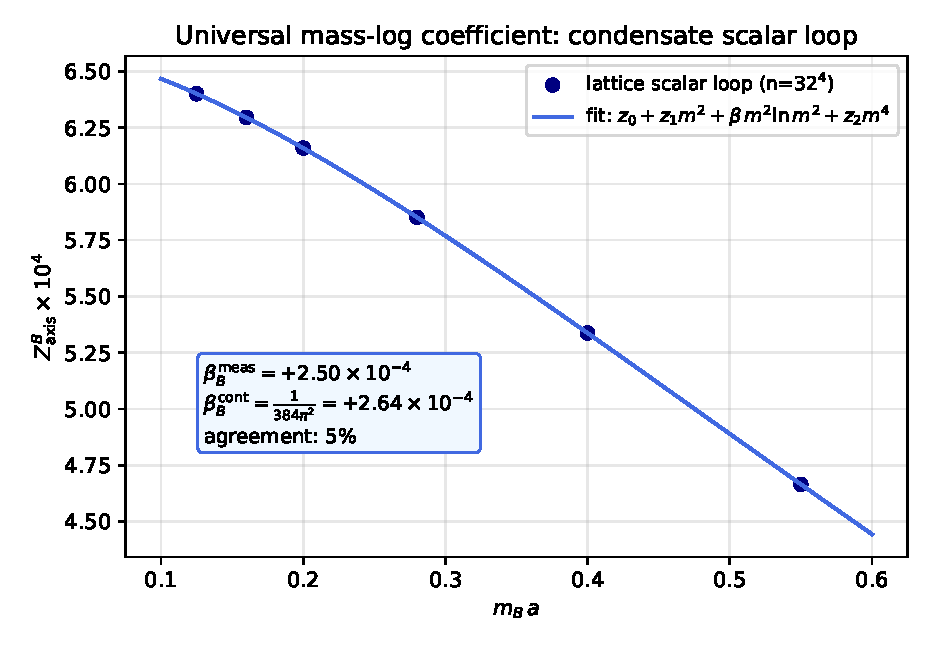
\includegraphics[width=0.7\columnwidth]{fig_mlog.pdf}
\caption{Mass scan of the axis transverse-traceless slope for the
condensate scalar loop.
The fitted universal coefficient of $m^2\ln m^2$ agrees with the
continuum heat-kernel prediction $1/(384\pi^2)$ to $5\%$,
validating the lattice extraction of the scheme-independent
(Sakharov-logarithmic) part of the induced gravitational action.}
\label{fig:mlog}
\end{figure}

\textbf{Finding 4: the induced non-minimal coupling and the
failure of the minimal survival condition.}
The non-minimal coupling of the condensate scalar is itself induced
by the fermion loop and is calculable by a chain-rule reduction:
since the fluctuation $\tilde\chi$ enters the fermion determinant
only through the mass, $m = y(v + \tilde\chi)$, the coefficient of
$\tfrac12\tilde\chi^2 R$ in the induced action is
\begin{equation}
\xi_{\mathrm{ind}}
= \tfrac12\,\frac{d^2 M^2_{\mathrm{ind}}}{d\tilde\chi^2}
= 4G\Bigl[\,Z'(m^2) + 2m^2 Z''(m^2)\Bigr]
= 2G\,\frac{d^2 Z}{dm^2}\Big|_{m},
\qquad G \equiv N y^2 ,
\label{eq:xichain}
\end{equation}
where $Z(m^2)$ is the (axis-TT) induced kinetic coefficient per
unit $4N$ studied above.
Inserting the universal logarithmic form
$Z \supset \beta_F\, m^2 \ln m^2$ gives the scheme-independent part
\begin{equation}
\xi_{\mathrm{ind}}\big|_{\mathrm{univ}}
= 4G\,\beta_F\,\bigl(3 - L\bigr),
\qquad L \equiv \ln\!\frac{\Lambda^2}{m^2}.
\label{eq:xiuniv}
\end{equation}
At the critical coupling, the prefactor collapses to a pure number.
With the continuum sharp-cutoff gap equation,
$G_c = 8\pi^2/\Lambda^2$, one finds the exact relation
$4G_c\beta_F = 4\cdot 8\pi^2/(192\pi^2) = 1/6$, hence
\begin{equation}
\xi_{\mathrm{ind}} = \tfrac{1}{6}\,(3 - L)
\qquad \text{(sharp-cutoff criticality)};
\label{eq:xi16}
\end{equation}
the lattice (Wilson, $r{=}1$) scheme gives
$G_c = 5.93$ (from $I_0 = 0.0844$, with an offset-grid cross-check
at the $1\%$ level), i.e.\ $4G_c\beta_F = 0.013$, an even smaller
prefactor.
The verdict is scheme-robust: the survival condition
$\xi_{\mathrm{eff}} > 1/6$ requires $L < 2$ in the most favorable
(sharp-cutoff) scheme---that is, $m_f > e^{-1}\Lambda \simeq
0.37\,\Lambda$---and is unattainable in the lattice scheme.
In the logarithmically induced regime $L \gg 1$, which is precisely
where the scheme-independent analysis is clean and where the
near-critical condensate naturally lives,
$\xi_{\mathrm{ind}} \simeq -\tfrac{1}{6}L < 0$: the induced
coupling runs \emph{away} from the survival region.
(A direct lattice extraction of $d^2Z/dm^2$ is contaminated by the
Wilson chiral artifacts---odd powers of $ma$ that vanish in the
continuum limit---so the statement rests on the validated universal
coefficient $\beta_F$; the chain rule itself is exact.)

We conclude that \emph{the minimal model fails its own survival
condition}: at leading order in $1/N$, the fermion and condensate
scalar sectors cannot self-generate a positive, scheme-independent
induced Newton constant.
Three routes remain within the framework:
(a) the vector channel, whose universal mass-logarithmic
coefficient has a different spin structure and is not yet computed;
(b) non-minimal microscopic operators (curvature-dependent
four-fermion couplings at the lattice scale), a model extension;
(c) treating $M_{\mathrm{Pl}}^2$ as a defining input fixed by the
counterterm condition, the conservative fallback consistent with
every result of this section.

\textbf{Finding 5: the vector channel reverses the sign.}
The framework's vector Hubbard--Stratonovich channel produces a
composite vector whose contact term supplies a tree-level mass: a
Proca-type massive vector (see the companion vector-channel paper
for the construction).
Heat-kernel analytics, anchored at the lattice-validated $2{:}1$
fermion-to-scalar point of the species table, predict for its
universal coefficient
$\beta_V = -3\beta_B$---\emph{opposite in sign} to all minimal
scalars and fermions.
We have subjected this to the lattice test by implementing a
lattice Proca field coupled to the background metric with the same
machinery (exact geometric coefficients
$\sqrt{g}\,g^{-1}\!\otimes g^{-1}$ and $\sqrt{g}\,g^{-1}$, forward
differences, numerical $h$-derivatives), validated by exact flat
eigenvalue structure $\{\hat s^2 + m^2\,(\times 3),\, m^2\}$, a
Sherman--Morrison propagator identity at the $10^{-15}$ level, and
the constant-$h$ effective action at the $10^{-8}$ level.
The longitudinal lattice mode has \emph{exactly} no kinetic term
(forward differences commute), realizing the compensating-scalar
structure of the Proca determinant at finite spacing.
The mass scan confirms the sign reversal decisively: the
vector-loop kinetic coefficient \emph{increases} with mass where
the scalar and fermion coefficients decrease, and every fit window
yields $\beta_V < 0$.
A homogeneous light-mass window ($m_V a = 0.11$--$0.20$, $n=32$)
gives
\begin{equation}
\beta_V = -7.2\times 10^{-4},
\qquad
\frac{\beta_V}{\beta_B}\Big|_{\mathrm{lat}} = -3.2(5),
\qquad
\frac{\beta_V}{\beta_B}\Big|_{\mathrm{analytic}} = -3,
\label{eq:betaVlat}
\end{equation}
consistent with the analytic prediction within extraction
systematics; the precision is limited by the longitudinal sector,
whose flat band at eigenvalue $m^2$ produces $1/m^2$-enhanced
$m^4\ln m^2$ lattice artifacts degenerate with the signal over
heavy-mass windows (windows including $m_V a \gtrsim 0.3$ drift to
ratios near $-5$).
A precision confirmation requires lighter masses on larger
lattices or a Stueckelberg-decomposed discretization; the sign,
which is the physically decisive property, is established.

\textbf{What survives, and what this means.}
The light-cone universality results are unaffected: the axis
isotropy of the kernel is exact (ten digits), as guaranteed by
$H(4)$ symmetry, and channel anisotropies remain confined to
dimension 6.
The degeneracy result reframes the central open problem of the
gravitational sector: the $\Lambda^2$-level normalization of
$M_{\mathrm{Pl}}^2$ is a defining condition of the microscopic
model, while the model's \emph{predictions} are the universal
mass-logarithmic coefficients---fermionic and condensate-bosonic,
the latter including the induced non-minimal coupling of the
composite scalar---together with the symmetry-protected light-cone
structure.
The universal coefficients are measured and benchmarked
(Finding 3); the induced non-minimal coupling is computed
(Finding 4) and the minimal fermion-plus-scalar content fails its
survival condition; and the vector channel is found to reverse the
sign (Finding 5), making the Proca composite the first species in
the framework that contributes positively to $M_{\mathrm{Pl}}^2$
at the scheme-independent level.
The priority calculations are now the precision lattice test of
$\beta_V/\beta_B = -3$ and the vector-channel gap analysis that
decides whether $m_V \ll \Lambda$ is dynamically realized.

\subsection{Status and scope}

The conclusions of this section are:
(i) the framework evades the radiative Lorentz-violation problem
\emph{if and only if} the substrate possesses a symmetry relating
the time direction to the spatial directions; the Euclidean
hypercubic lattice provides such a symmetry, and we therefore adopt
it as a defining structural assumption of the model, with the
real-time theory defined by analytic continuation;
(ii) under this assumption, speed universality at dimension 4 holds
to all orders in $1/N$ by the symmetry classification, and the
residual channel-dependent violation is of dimension-6 size,
Eq.~\eqref{eq:dc-dim6}, far below current bounds;
(iii) the explicit one-loop verification covers both the scalar
channel and the graviton (stress-tensor) channel; the
Ward-complete graviton analysis (Section~\ref{sec:ttcheck})
additionally reveals induced non-covariant local terms and a
negative covariant kinetic coefficient at leading order in $1/N$
for the minimal prescription, sharpening the open problem of the
induced Newton constant.


% ===================================================================
\section{Weinberg--Witten Evasion}
\label{sec:WW}
% ===================================================================

The Weinberg--Witten theorem \cite{Weinberg:1980kq} states that in
a theory with a conserved, Lorentz-covariant energy-momentum
tensor, there are no massless particles of spin $> 1$ that are
composites of the fields carrying that tensor.
Since the emergent graviton is built from fermion stress-tensor
correlations, the theorem appears to forbid its existence.

The theorem's hypotheses, however, require \emph{exact} Lorentz
covariance and exact conservation at all scales.
On the lattice, both fail at the UV scale: Lorentz symmetry is
broken by the discretization, and stress-tensor conservation holds
only up to dimension-$\geq 6$ Symanzik operators,
Eq.~\eqref{eq:Ward}.
At the scale where the composite graviton is assembled
($p \sim \Lambda$), the WW hypotheses do not apply; as
$p/\Lambda \to 0$, Lorentz invariance and conservation are restored
to accuracy $(p/\Lambda)^2$, and the graviton propagates as a
standard massless spin-2 particle.
This is the mechanism identified by Volovik
\cite{Volovik:2003fe} in condensed-matter analogues.

Section~\ref{sec:lightcone} is what elevates this argument beyond
power counting: the $(p/\Lambda)^2$ suppression survives radiative
corrections \emph{because} of the $H(4)$ symmetry of the substrate,
not merely because of the classical dimension of the breaking
operators.
Observable Lorentz violation is then bounded by
$\delta_{\mathrm{LV}} \sim (E/\Lambda)^2 \lesssim
(E/M_{\mathrm{Pl}})^2$, i.e.\ $\lesssim 10^{-30}$ for
$E \lesssim 10^4$~GeV, far below bounds from gamma-ray
time-of-flight and gravitational-wave observations
\cite{Fermi:2009,LIGO:2017}.


% ===================================================================
\section{Newtonian Limit}
\label{sec:newton}
% ===================================================================

In the weak-field, non-relativistic limit, the linearized
Einstein equation sourced by a static mass distribution
$T^{00} = \rho(\mathbf{r})$ yields
\begin{equation}
\nabla^2 \Phi_N = 4\pi G\,\rho,
\qquad
\Phi_N(\mathbf{r}) = -G\int d^3r'\,
\frac{\rho(\mathbf{r}')}{|\mathbf{r} - \mathbf{r}'|},
\label{eq:Poisson}
\end{equation}
with $G$ fixed by the induced Planck mass, Eq.~\eqref{eq:Mpl}.
This confirms that the induced gravitational sector reproduces
standard Newtonian gravity in the appropriate limit.

Combined with the angular-mode identification of
Section~\ref{sec:angular} and the phenomenology of
Ref.~\cite{Cheng:2025sparc}, the lattice fermion framework
produces both gravitational dynamics (induced sector) and
ultralight dark-matter phenomenology (angular condensate mode)
from the same microscopic Lagrangian~\eqref{eq:L0}.


% ===================================================================
\section{Discussion and Conclusions}
\label{sec:discuss}
% ===================================================================

\subsection{Summary of the derivation chain}

\begin{enumerate}
\item \textbf{Microscopic input}: NJL Lagrangian on a Planck-scale
  Euclidean hypercubic lattice (Eq.~\ref{eq:L0}); the hypercubic
  symmetry is a structural requirement
  (Section~\ref{sec:lightcone}).
\item \textbf{Vacuum}: Real condensate at the minimum of the
  one-loop angular potential; substrate fermions gapped at
  $\mathcal{O}(\Lambda)$, hence unobservable
  (Section~\ref{sec:vacuum}).
\item \textbf{Light sector}: Angular pseudo--Goldstone mode with
  naturally small mass $m_\theta^2 \sim \varepsilon\Lambda^2$,
  identified with the ultralight dark-matter scalar of
  Ref.~\cite{Cheng:2025sparc} (Section~\ref{sec:angular}).
\item \textbf{Induced gravity}: External-metric coupling
  $\to$ stress-tensor correlators $\to$ approximate Ward identities
  $\to$ TT spin-2 projection $\to$ Fierz--Pauli $\to$
  Einstein--Hilbert via Deser iteration; induced
  $M_{\mathrm{Pl}}^2 \sim N\Lambda^2/8\pi^2$
  (Section~\ref{sec:induced}).
\item \textbf{Radiative light-cone stability}: $H(4)$ symmetry
  protects speed universality at dimension 4 to all orders in
  $1/N$; verified at one loop; without the symmetry the splitting
  is $\mathcal{O}(1)$ (Section~\ref{sec:lightcone}).
\item \textbf{WW evasion and Newtonian limit}: established in
  Sections~\ref{sec:WW}--\ref{sec:newton}.
\end{enumerate}

Each step uses standard techniques (HS linearization, large-$N$,
heat-kernel expansion, Ward identities, Fierz--Pauli theory, Deser
self-coupling, lattice perturbation theory).
The contributions of this paper are
(a) the corrected vacuum analysis, replacing the untenable
``imaginary vacuum'' hypothesis with a real condensate plus a
naturally light angular mode,
(b) the consistent induced-gravity formulation of the tensor
sector, and
(c) the light-cone stability theorem and its explicit verification,
which directly answers the radiative Lorentz-violation objection of
Collins et al.

\subsection{Assumptions and open problems}

\begin{itemize}
\item \textbf{Lattice spacing at the Planck length.}
  Assumed, with no independent justification beyond dimensional
  consistency.
\item \textbf{Induced cosmological constant.}
  The leading induced term $c_0 N \Lambda^4$ must be cancelled by a
  bare counterterm to obtain a near-flat background.
  This is the cosmological constant problem in its standard
  induced-gravity form; we do not solve it.
  The masslessness of the emergent graviton requires no tuning
  beyond this one.
\item \textbf{Normalization of the induced Newton constant
  (defining condition).}
  The full structure analysis (Section~\ref{sec:ttcheck}) shows
  that the quadratically divergent part of the induced Newton
  constant is counterterm-convention-dependent---an exact
  degeneracy between covariant and non-covariant local structures.
  $M_{\mathrm{Pl}}^2$ at this order is therefore an input of the
  model; the predictive, scheme-independent content is the
  universal mass-logarithmic induced contribution, now measured and
  benchmarked (Finding 3): minimal matter contributes negatively,
  and the induced non-minimal coupling computed in Finding 4 fails
  the survival condition $\xi_{\mathrm{eff}} > 1/6$ in the clean
  regime.
  Remaining in-model routes: the vector channel, non-minimal
  microscopic operators, or $M_{\mathrm{Pl}}^2$ as a defining
  input.
\item \textbf{Composite spin-2 pole.}
  The Ward structure supports, but does not nonperturbatively
  establish, a genuine massless spin-2 pole in
  $\langle TT\rangle$; the decisive test is a lattice measurement
  of the Barnes--Rivers--projected stress-tensor correlator.
\item \textbf{Coupling of the angular mode to baryons.}
  The monopole coupling used phenomenologically in
  Ref.~\cite{Cheng:2025sparc} must be induced through explicit
  breaking and/or radial-mode mixing; the quantitative chain is
  open.
\item \textbf{Non-covariant lattice counterterms.}
  The induced action contains non-covariant local terms at cutoff
  order (Section~\ref{sec:ttcheck}); the covariance-restoring
  counterterm structure has been identified at $\mathcal{O}(q^2)$
  for axis-projected quantities, but a structure-complete
  classification at $\mathcal{O}(q^4)$ and for general
  discretization prescriptions is deferred.
\end{itemize}

\subsection{Relation to existing approaches}

The framework combines elements of several programmes:
Sakharov induced gravity \cite{Sakharov:1967pk} (here with a
definite UV substrate that renders the induced coefficients
computable), Volovik's emergent-symmetry mechanism
\cite{Volovik:2003fe} (here with an explicit particle-physics
Lagrangian and a proof of radiative light-cone stability), and
NJL/composite-boson technology
\cite{Nambu:1961tp,Akama:1978pg,Zee:1981,Amati:1982bp}
(here applied to the condensate and dark-matter sector rather than
to the graviton itself).

\subsection{Future directions}

(i) computing the vector channel's universal mass-logarithmic
coefficient, the remaining in-model route to a positive induced
Newton constant;
(ii) the Barnes--Rivers--projected $\langle TT\rangle$ correlator
beyond one loop, testing for a genuine composite spin-2 pole;
(iii) the explicit-breaking chain fixing the angular-mode coupling
to baryons, connecting $\varepsilon$ to the SPARC-scale
phenomenology of Ref.~\cite{Cheng:2025sparc};
(iv) the antisymmetric-tensor (torsion) and vector/axial (gauge)
sectors;
(v) cosmological implications of the condensate energy budget,
where the cosmological constant problem must be confronted.


% ===================================================================
\section*{Acknowledgments}
% ===================================================================

The author acknowledges the use of large language models
(Claude, Anthropic) as a research-assistance tool during this work,
including assistance with the vacuum phase-structure analysis, the
Ward identity chain, the one-loop lattice computations of
Section~\ref{sec:lightcone}, and manuscript editing.
All physical ideas and the model construction are the author's own;
all derivations and numerical results were reviewed and verified by
the author, who takes full responsibility for the content of the
manuscript.


% ===================================================================
\begin{thebibliography}{99}

\bibitem{Sakharov:1967pk}
A.~D.~Sakharov,
``Vacuum Quantum Fluctuations in Curved Space and the Theory of
Gravitation,''
\textit{Sov.\ Phys.\ Dokl.}\ \textbf{12}, 1040 (1968).

\bibitem{Volovik:2003fe}
G.~E.~Volovik,
\textit{The Universe in a Helium Droplet}
(Oxford University Press, 2003).

\bibitem{Barcelo:2005fc}
C.~Barcel\'{o}, S.~Liberati, and M.~Visser,
``Analogue Gravity,''
\textit{Living Rev.\ Rel.}\ \textbf{8}, 12 (2005).

\bibitem{Nambu:1961tp}
Y.~Nambu and G.~Jona-Lasinio,
``Dynamical Model of Elementary Particles Based on an Analogy
with Superconductivity.\ I,''
\textit{Phys.\ Rev.}\ \textbf{122}, 345 (1961).

\bibitem{Nambu:1961fr}
Y.~Nambu and G.~Jona-Lasinio,
``Dynamical Model of Elementary Particles Based on an Analogy
with Superconductivity.\ II,''
\textit{Phys.\ Rev.}\ \textbf{124}, 246 (1961).

\bibitem{Hubbard:1959ub}
J.~Hubbard,
``Calculation of Partition Functions,''
\textit{Phys.\ Rev.\ Lett.}\ \textbf{3}, 77 (1959).

\bibitem{Stratonovich:1957}
R.~L.~Stratonovich,
``On a Method of Calculating Quantum Distribution Functions,''
\textit{Sov.\ Phys.\ Dokl.}\ \textbf{2}, 416 (1957).

\bibitem{tHooft:1973alw}
G.~'t~Hooft,
``A Planar Diagram Theory for Strong Interactions,''
\textit{Nucl.\ Phys.\ B} \textbf{72}, 461 (1974).

\bibitem{Coleman:1985rnk}
S.~Coleman,
\textit{Aspects of Symmetry}
(Cambridge University Press, 1985).

\bibitem{Akama:1978pg}
K.~Akama,
``An Attempt at Pregeometry: Gravity with Composite Metric,''
\textit{Prog.\ Theor.\ Phys.}\ \textbf{60}, 1900 (1978).

\bibitem{Zee:1981}
A.~Zee,
``Broken-Symmetric Theory of Gravity,''
\textit{Phys.\ Rev.\ Lett.}\ \textbf{42}, 417 (1979).

\bibitem{Amati:1982bp}
D.~Amati and G.~Veneziano,
``A Unified Gauge and Gravity Theory with Only Matter Fields,''
\textit{Nucl.\ Phys.\ B} \textbf{204}, 451 (1982).

\bibitem{Weinberg:1980kq}
S.~Weinberg and E.~Witten,
``Limits on Massless Particles,''
\textit{Phys.\ Lett.\ B} \textbf{96}, 59 (1980).

\bibitem{Fierz:1939ix}
M.~Fierz and W.~Pauli,
``On Relativistic Wave Equations for Particles of Arbitrary Spin
in an Electromagnetic Field,''
\textit{Proc.\ Roy.\ Soc.\ Lond.\ A} \textbf{173}, 211 (1939).

\bibitem{Deser:1969wk}
S.~Deser,
``Self-Interaction and Gauge Invariance,''
\textit{Gen.\ Rel.\ Grav.}\ \textbf{1}, 9 (1970).

\bibitem{Collins:2004bp}
J.~Collins, A.~Perez, D.~Sudarsky, L.~Urrutia, and H.~Vucetich,
``Lorentz invariance and quantum gravity: an additional
fine-tuning problem?,''
\textit{Phys.\ Rev.\ Lett.}\ \textbf{93}, 191301 (2004).

\bibitem{Liberati:2013xla}
S.~Liberati,
``Tests of Lorentz invariance: a 2013 update,''
\textit{Class.\ Quantum Grav.}\ \textbf{30}, 133001 (2013).

\bibitem{Caracciolo:1989pt}
S.~Caracciolo, G.~Curci, P.~Menotti, and A.~Pelissetto,
``The energy-momentum tensor for lattice gauge theories,''
\textit{Annals Phys.}\ \textbf{197}, 119 (1990).

\bibitem{Visser:2002ew}
M.~Visser,
``Sakharov's induced gravity: a modern perspective,''
\textit{Mod.\ Phys.\ Lett.\ A} \textbf{17}, 977 (2002).

\bibitem{Hui:2016ltb}
L.~Hui, J.~P.~Ostriker, S.~Tremaine, and E.~Witten,
``Ultralight scalars as cosmological dark matter,''
\textit{Phys.\ Rev.\ D} \textbf{95}, 043541 (2017).

\bibitem{Cheng:2025sparc}
Z.~H.-H.~Cheng,
``Emergent Yukawa Dark Matter Halos from a Lattice Fermion
Condensate: Fits to 175 SPARC Galaxies,''
in preparation (2025).

\bibitem{LIGO:2017}
B.~P.~Abbott \textit{et al.} (LIGO/Virgo),
``GW170817: Observation of Gravitational Waves from a Binary
Neutron Star Inspiral,''
\textit{Phys.\ Rev.\ Lett.}\ \textbf{119}, 161101 (2017).

\bibitem{Fermi:2009}
A.~A.~Abdo \textit{et al.} (Fermi LAT/GBM),
``A limit on the variation of the speed of light arising from
quantum gravity effects,''
\textit{Nature} \textbf{462}, 331 (2009).

\end{thebibliography}

\end{document}
